\section{Komponenten}
\begin{frame}{Komponenten}

\begin{overprint}
\onslide<1> \begin{center}\includegraphics[height=0.8\textheight]{imgs/komponenten_1.pdf}\end{center}
\onslide<2> \begin{center}\includegraphics[height=0.8\textheight]{imgs/komponenten_2.pdf}\end{center}
\onslide<3> \begin{center}\includegraphics[height=0.8\textheight]{imgs/komponenten_3.pdf}\end{center}
\onslide<4> \begin{center}\includegraphics[height=0.8\textheight]{imgs/komponenten_4.pdf}\end{center}
\onslide<5> \begin{center}\includegraphics[height=0.8\textheight]{imgs/komponenten_5.pdf}\end{center}
\end{overprint}

\end{frame}

\begin{frame}{Microsoft Kinect/OpenNI}
	\begin{itemize}
	\item Eigentlich: Interaktion mit XBox360 für Spiele
	\item Mit OpenNI Framework Interaktion mit PC programmierbar
	\item Erkennt "`Skelett"' eines Benutzers
		\begin{itemize}
		\item Positionen einzelner Körperteile kann ermittelt werden
		\item z.B. Hand, Torso, Bein
		\end{itemize}
	\end{itemize}
\end{frame}

\begin{frame}{Microsoft Kinect/OpenNI}
\begin{center}
	\includegraphics[height=0.8\textheight]{imgs/multiplayer.jpg}
\end{center}
\end{frame}

\begin{frame}{Positionsbestimmung}
\begin{itemize}
\item OpenNI berechnet Abstände zu Eingabegerät in mm $(x,y,z)$
\item Koordinatensystem an Benutzer anpassen
	\begin{itemize}
	\item $x=x_{Hand}-x_{Torso}$
	\item $y=y_{Hand}-y_{Torso}$
	\item $z=z_{Hand}-z_{Torso}$
	\end{itemize}
\item Koordinatensystem zur besseren Bedienung um 200mm in $x$- und $z$-Richtung verschoben
\end{itemize}
\end{frame}

\begin{frame}{Greifarm}
\begin{itemize}
\item Greifarm wird über COM-Port angesteuert
\item Für jeden Servomotor am Greifarm wird ein Winkel übertragen (etwa 0-1)
\item 6 Servomotoren werden angesteuert
\item Ansteuerung über "`API"'
	\begin{itemize}
	\item Frühere Projekte steuern Greifarm an
	\item Anpassung an unsere Aufgabenstellung
	\end{itemize}
\end{itemize}
\end{frame}